\section{Evaluation}
We evaluate \mimovl{} across 50 tasks to comprehensively assess its capabilities. Appendix~\ref{sec:eval_bench} lists all the benchmarks adopted in our evaluation. 
We also assess model performance with an in-house evaluation set. 






\begin{table}[htbp]
    \centering
    \small
    \resizebox{0.99\textwidth}{!}{
    \begin{tabular}{l c | S[table-format=2.1] S[table-format=2.1] | S[table-format=2.1] S[table-format=2.1] S[table-format=2.1] | S[table-format=2.1] S[table-format=2.1]}
    \toprule
    \multirow{2}{*}{\textbf{Benchmark}}  &  \multirow{2}{*}{\textbf{Metrics}} & \textbf{MiMo-VL} & \textbf{MiMo-VL} & \textbf{Qwen2.5-VL} & \textbf{InternVL3} & \textbf{Gemma-3}  & \multicolumn{1}{c}{\multirow{2}{*}{\textbf{GPT-4o}}} & \multicolumn{1}{c}{{\textbf{Claude 3.7}}} \\
    & & \textbf{7B-SFT} & \textbf{7B-RL} & \textbf{7B} & \textbf{8B} & \textbf{27B-IT} &   & \textbf{Sonnet} \\
    \midrule
    \rowcolor{xiaomiorange!20}
    \multicolumn{9}{l}{\textbf{General}} \\ %
    MMMU$_{\mathrm{val}}^{\dag}$          & Acc.         & 64.6  & \textbf{66.7} & 58.6  & 62.7  & 64.9  &   70.7   & 69.8*                \\
    MMMU-Pro$_{\mathrm{standard}}$        & Acc.         & 45.2  & \textbf{46.2} & 34.7* & 45.6* & 37.8* &  42.5*   &  56.5*               \\
    MMMU-Pro$_{\mathrm{vision}}$          & Acc.         & 39.4  & \textbf{40.3} & 29.4* & 37.8* & 24.9* &    36.1*    &  45.8*               \\
    MMBench-en$_{\mathrm{test}}$          &  Acc.        &     \textbf{84.5}  & 84.4 & 83.5  & 83.4  &    81.6*   &    84.6*    &  84.8*               \\
    MMBench-cn$_{\mathrm{test}}$          &  Acc.        &      81.9 & 82.0  & \textbf{83.4} & 82.2  &    82.4*   &    84.5*    &  83.7*               \\
    Mantis                                &  Acc.        & \textbf{78.8} & 78.3  & 74.7* & 72.8* &    70.0*   &  75.6* &  75.1*               \\
    MME-RealWorld$_{\mathrm{en}}$         &  Acc.        & 57.4  & \textbf{59.1} & 57.4  & 56.1* &   51.9*    &    57.5*    &  50.8*               \\
    MME-RealWorld$_{\mathrm{cn}}$         &  Acc.        & 55.0  & 55.5  & 51.2* & \textbf{58.5}* &  47.9*     &    58.5*   &  40.6*               \\
    AI2D                                  &  Acc.        &  83.2 & 83.5 & 83.9  & \textbf{85.2}  & 84.5  &  82.6* &  81.4*               \\ 
    BLINK$_{\mathrm{val}}$                &  Acc.        &  \textbf{62.5} & 62.4 & 56.4  & 55.5  & 53.3* &  60.0  &  62.3*               \\ 
    CV-Bench                              & Acc.         &  81.8 & \textbf{82.3} & 75.4* & 81.0* & 70.4* &  76.0* & 75.4* \\ 
    VibeEval$^{\dag}$                      &  GPT-Score   & 47.2  & \textbf{54.7} & 47.7* & 43.6* & 44.0* & 64.7  &  39.0*               \\ 
    VL-RewardBench$^{\dag}$                &  Macro Acc.  &  61.9 & \textbf{62.7} & 47.3* & 49.7* & 51.9* &  62.4  & 67.4*                \\ 
    V* &  Acc.        &  80.6 & \textbf{81.7} & 73.8* & 72.8* & 50.8* &  73.9  &  {-}               \\  
    VLMs are Blind                        &  Acc.        & 78.0  & \textbf{79.4} & 37.4* & 36.8* &  18.6*     &   49.8*   &  72.1*               \\ 
    PixmoCount                            &  Acc.        &  \textbf{79.4} & \textbf{79.4} & 60.7* & 62.0  &   48.6*    &    54.4*  &  53.5*               \\ 
    CountBench                            &  Acc.        & 87.0  & \textbf{90.4} & 74.1* & 80.0* & 77.2*  &   85.7* &  90.2*               \\ 
    RefCOCO$_{\mathrm{val}}^\mathrm{avg}$              &  Acc.@0.5    & 85.7  & 89.6  & 87.1  & \textbf{90.1} &   {-}    &  {-}      &   {-}              \\  
    \midrule
    \rowcolor{xiaomiorange!20}
    \multicolumn{9}{l}{\textbf{Doc \& OCR}} \\ %
    ChartQA$^{\dag}$                      &  Acc.        & \textbf{92.9} & 91.7  & 90.2* & 89.6* & 78.0  &  86.7  & 92.2*                 \\
    CharXiv$_{\mathrm{RQ}}^{\dag}$        &  Acc.        & 54.4  & \textbf{56.5} & 42.5  & 37.6  &  29.2*     &  52.0 &   63.0*              \\
    CharXiv$_{\mathrm{DQ}}^{\dag}$        &  Acc.        &  \textbf{87.0} & 86.8  & 73.9  & 73.6  &   63.8*    &  86.5  &   89.5*              \\
    DocVQA$_{\mathrm{val}}^{\dag}$        &  Acc.        &  95.2 &   \textbf{95.7}    & 95.5* & 89.4* & 86.6  &    93.0*    &   94.1*              \\
    InfoVQA$_{\mathrm{val}}^{\dag}$       &  Acc.        & 87.2  & \textbf{88.0} & 81.4* & 70.7* & 70.6  &  82.1*  &    65.5*             \\
    SEED-Bench-2-Plus                     &  Acc.        & 71.9  & \textbf{72.4} & 70.7  & 69.7  &   66.3*    &   71.1*  & 72.9*                \\
    OCRBench$^{\dag}$                     &  Acc.        & 87.6  & 86.6  & \textbf{89.7}* & 88.0  &   77.6*    & 84.3*  &  80.6*               \\
    \midrule
    \rowcolor{xiaomiorange!20}
    \multicolumn{9}{l}{\textbf{GUI}} \\ %
    VisualWebBench$_{\mathrm{avg}}$       &  Acc.        &  \textbf{80.2} & \textbf{80.2}  & 72.9* & 62.7  &    49.7*   & 80.2  &  79.3*               \\
    WebSrc$_{\mathrm{val}}$               &  SQuAD F1    &  \textbf{96.5} & 95.3  & 94.6* & 91.1  &    89.0*   & 89.1*   & 91.1*                \\
    ScreenSpot                            & Center Acc.  &  \textbf{87.3} & 87.2  & 84.7  & 79.5  &   {-}    & 18.3   &  {-}               \\
    ScreenSpot-v2                         & Center Acc.  & 89.5  & \textbf{90.5} & 88.0  & 81.4  &   {-}    & 18.5   &  {-}               \\
    ScreenSpot-Pro$_{\mathrm{avg}}$                & Center Acc.  & 39.9  & \textbf{41.9} & 29.0  &  {-}  &   {-}    & {-}    &   {-}              \\
    OSWorld-G$_{\mathrm{no\_refusal}}$    & Center Acc.  &  54.7 & \textbf{56.1} & 37.5* &  {-}  &   {-}    & {-}    &   {-}              \\
    \midrule
    \rowcolor{xiaomiorange!20}
    \multicolumn{9}{l}{\textbf{Video}} \\ %
    Video-MME$_{\mathrm{w/o~sub.}}$                             & Acc.         & 66.9  & \textbf{67.4} & 65.1 & 66.3  &    {-}   & {-}    &     {-}            \\
    Video-MMMU                            & Acc.         &  \textbf{53.1} &   43.3   & 47.4  &   48.9*    &   {-}    & {-}    &    {-}             \\
    EgoSchema$_{\mathrm{val}}$                             & Acc.         & 60.4  & 59.6  & 62.4* &   \textbf{68.2}*   &   {-}   & {-}    &    {-}             \\
    Charades-STA                          & mIoU         &   38.5    & \textbf{50.0} & 43.6  &   25.4    &    {-}   & {-}    &  {-}               \\
    \midrule
    \rowcolor{xiaomiorange!20}
    \multicolumn{9}{l}{\textbf{Text}} \\ %
    GPQA Diamond                          & Pass@1       & 56.3 & \textbf{58.3} & 30.3* & 33.5* & 40.9  & 50.6* & 66.0* \\
    SuperGPQA                             & Pass@1       & 42.6 & \textbf{44.3}      & 25.4* & 29.4* & 29.3* & 31.6* & 54.4* \\
    DROP                                  & 3-shot F1    & 82.7 & \textbf{85.1} & 67.6* & 77.5* & 72.2  & 81.5  & 87.2* \\
    MMLU-Pro                              & EM           & 59.8 &  \textbf{64.8}     & 48.7* & 58.3* & 45.3  & 69.1  & 81.0  \\
    IF-Eval                               & Prompt Strict& 75.3 &   75.9    & 75.1* & 87.2* & \textbf{88.9} & 82.5  & 88.7* \\
    \bottomrule
    \end{tabular}
}
    \caption{
        Comparison of \mimovl{} models with other models on diverse visual-language and text benchmarks.
        Results marked with * are obtained using our evaluation framework. $^{\dag}$ indicates that evaluation is performed using GPT-4o. The best results among open-source models are \textbf{bolded}.
    }
    \label{tab:general_updated} %
\end{table}





    
    







   
   









\subsection{Evaluation Setting}


For image understanding benchmarks, we set the max pixels for the input image to 4096 × 28 × 28 and the maximum generation tokens to 32,768, employing greedy search for decoding. 
For video benchmarks, videos are sampled at 2 FPS, with a maximum of 256 frames and a total token limit of 16,384.
For text evaluation benchmarks, we set the max new tokens for generation as 32,768, temperature as 0.6 and top-p as 0.95.
We adapt the existing framework based on LMMs-Eval~\citep{lmmseval} to better accommodate long-CoT reasoning models. 
We further optimize the evaluation logic for specific tasks to ensure better evaluation consistency. 
To facilitate open research, we open-source our evaluation framework with all prompts used.\footnote{\url{https://github.com/XiaomiMiMo/lmms-eval}}


\subsection{General Capabilities}


Table~\ref{tab:general_updated} presents benchmark results assessing the general capabilities of VLMs. Our \mimovl{} models demonstrate consistently leading performance across a diverse range of vision-language and text benchmarks, establishing new state-of-the-art results among open-source models and even surpassing proprietary counterparts.

Specifically, our \mimovl{} models achieve state-of-the-art results among open-source models. \mimovlsft{} and
\textbf{(i)} On general vision-language tasks, our models achieve exceptional performance that leads the open-source field. \mimovlsft{} and \mimovlrl{} obtain 64.6\% and 66.7\% on MMMU$_{\mathrm{val}}$ respectively, outperforming much larger models such as Gemma 3 27B. For document and chart understanding, \mimovlrl{} excels with a top open-source score of 56.5\% on CharXiv$_{\mathrm{RQ}}$, significantly exceeding Qwen2.5-VL (42.5\%) by 14.0 points and InternVL3 (37.6\%) by 18.9 points.
\textbf{(ii)} Our models demonstrate superior video understanding capabilities while maintaining strong textual performance. 
MiMo-VL-SFT achieves a leading 53.1\% on Video-MMMU, and MiMo-VL-RL obtains an impressive 50.0\% mIoU on Charades-STA. \textbf{(iii)} Compared with \mimo{}, our models maintain decent performance on text-only benchmarks.
\textbf{(iv)} Remarkably, our MoRL yields comprehensive improvements, with the most impressive gains observed on challenging benchmarks such as VibeEval and CountBench. 




\begin{table}[t]
    \centering
    \small
    \sisetup{table-align-text-post=false} %
    \resizebox{\textwidth}{!}{%
    \begin{tabular}{l c | S[table-format=2.1] S[table-format=2.1] | S[table-format=2.1] S[table-format=2.1] S[table-format=2.1] S[table-format=2.1] | S[table-format=2.1] S[table-format=2.1]}
    \toprule
    \textbf{Reasoning}  &  \multirow{2}{*}{\textbf{Metrics}} & {\textbf{MiMo-VL}} & {\textbf{MiMo-VL}} & {\textbf{QVQ-72B}} & {\textbf{Qwen2.5-VL}} & {\textbf{Intern-VL3}} & {\textbf{Qwen2.5}}  & \multicolumn{1}{c}{\multirow{2}{*}{\textbf{GPT-4o}}} & {\textbf{Gemini-2.5}} \\
    \textbf{Benchmark} & & {\textbf{7B-SFT}} & {\textbf{7B-RL}} & {\textbf{Preview}} & {\textbf{72B}} & {\textbf{78B}} & {\textbf{72B}} &  & {\textbf{Pro}} \\
    \midrule
    \rowcolor{xiaomiorange!20}
    \multicolumn{10}{l}{\textbf{Multi-modal}} \\ %
    OlympiadBench  & Acc.  & \textbf{59.4} & \textbf{59.4} & 20.4  & 37.2{*}  & 12.3 & {{-}} &  25.9 & 69.8   \\  
    MathVision     &  Acc. & 57.9 & \textbf{60.4} & 35.9 & 38.1    & 43.2 & {{-}} & 31.2  & 69.1    \\  
    MathVerse$_{\mathrm{vision\_only}}^{\dag}$  & Acc. & 67.1 & \textbf{71.5} & 45.1{*} & 57.6 & 51.0 & {{-}} & 49.9  &  76.7    \\  
    DynaMath         & Worst-case Acc. & \textbf{46.9}  & 45.9  & 30.7  & 38.1{*} & 35.1 & {{-}} & 48.5 & 56.3   \\
    WeMath & Strict Score & 65.1 & \textbf{66.3} & 37.7{*}  & 50.6{*} & 46.1& {{-}} & 50.6  & 78.0   \\
    LogicVista & Acc. & 61.2 & \textbf{61.4} & 53.8{*}  & 57.1{*}  & 55.9 & {{-}} & 64.4 & 73.8   \\
    MathVista$_{\mathrm{mini}}^{\dag}$ &  Acc. & \textbf{81.8} & 81.5 & 71.4  & 74.8 & 72.2 & {{-}} & 63.8  & 80.9    \\
    \midrule
    \rowcolor{xiaomiorange!20}
    \multicolumn{10}{l}{\textbf{Text}} \\ %
    MATH500 & Pass@1         & 95.0& \textbf{95.4} & 83.8{*} & 83.0 & 68.8{*} & 82.8{*} & 78.2{*} & 95.2 \\
    AIME24 & Pass@1   & 66.4 & \textbf{67.5} & 25.2{*} & 16.7{*} & 12.2{*} & 19.4{*} & 10.9{*} & 92.0  \\
    AIME25 & Pass@1   & 50.9 & \textbf{52.5} & 18.1{*} & 10.8{*} & 11.7{*} & 13.3{*} & 8.7{*}  & 86.7  \\
    \bottomrule
    \end{tabular}%
    }
    \caption{
        Comparison of \mimovl{} with other models on reasoning benchmarks.
        Results marked with * are obtained using our evaluation framework. $^{\dag}$ indicates that evaluation is performed using GPT-4o. The best results among open-source models are \textbf{bolded}.
    }
    \label{tab:reason_modified_final} %
\end{table}



















\subsection{Reasoning Tasks}

Table~\ref{tab:reason_modified_final} presents evaluation results for multimodal and text reasoning benchmarks.
In multimodal reasoning, both the SFT and RL models significantly outperform all compared open-source baselines across these benchmarks.
Notably, \mimovlsft{} surpasses much larger models, including Qwen2.5-VL-72B and QVQ-72B-Preview.
The RL model further improves performance on most reasoning benchmarks.
For example, \mimovlrl{} boosts accuracy on MathVision from 57.9\% to 60.4\%.
\mimovl{} models also exhibit impressive reasoning capabilities on pure text benchmarks, even outperforming Qwen2.5-72B.
These results demonstrate that our multimodal pre-training and post-training recipes effectively endow the model with exceptional visual capabilities and strong text intelligence.





\subsection{GUI Tasks}

\begin{figure}[t]
    \centering
    \includegraphics[width=0.98\linewidth]{figures/mimo-gui-v3.pdf}
    \caption{GUI understanding and grounding results. \mimovlrl{} achieves comparable results with GUI specialized models.}
    \label{fig:gui_specific}
\end{figure}

In addition, we demonstrate that \mimovl{} models possess exceptional GUI understanding and grounding capabilities. 
In Table~\ref{tab:general_updated}, \mimovlrl{} outperforms all other general VLMs compared. In Figure~\ref{fig:gui_specific}, we further compare \mimovlrl{} with GUI-specialized models (UI-TARS-1.0~\citep{qin2025ui}, Aguvis~\citep{xu2024aguvis}, OS-Atlas~\citep{wu2024atlas}) of similar size on GUI Understanding (WebSrc, VisualWebBench) and Grounding (Screenspot, Screenspot-v2, Screenspot-Pro, OSWorld-G) benchmarks. As a general-purpose VLM, MiMo-VL achieves comparable or even superior performance to GUI-specialized models, particularly on the more challenging Screenspot-Pro and OSWorld-G benchmarks.

\begin{figure}
    \centering
    \includegraphics[width=\linewidth]{figures/elo_rating.pdf}
    \caption{Elo ratings comparison across VLMs. \mimovlrl{} achieves the highest rating among open-source models, approaching the performance of proprietary alternatives such as Claude 3.7 Sonnet.}
    \label{fig:elo_rating}
\end{figure}

\begin{figure}
    \centering
    \includegraphics[width=0.95\linewidth]{figures/mimo_7b_sft_training_curves.pdf}
    \caption{\mimovlsft{} training curves in Stage 4.}
    \label{fig:mimo_7b_sft_performance}
\end{figure}

\begin{figure}[t!]
    \centering
    \includegraphics[width=0.6\linewidth]{figures/mimo_7b_vl_onpolicy_offpolicy_rl_aime24_25.pdf}
    \caption{On-policy RL and vanilla GRPO shows contrasting scaling behavior: on-policy RL performance continuously improves with more data, while vanilla GRPO reaches a plateau around 20,000 samples.}
    \label{fig:onpolicyrl}
\end{figure}



\subsection{Elo Rating}
Inspired by ChatbotArena~\citep{zheng2023chatbotarena}, we construct a balanced bilingual (Chinese and English) in-house evaluation dataset comprising real user prompts. This approach assesses user preference beyond traditional benchmark scores, providing insights into practical model performance in real-world scenarios.

Following the methodology of \citep{Chou2024VisionArena2R}, we conduct pairwise comparisons between \mimovl{} and competing models, including leading proprietary models and open-source VLMs ranging from 7B to 72B parameters. We compute Elo ratings based on GPT-4o judgments with style-controlled evaluation protocols. 
Our evaluation covers a diverse range of visual-linguistic tasks, including multimodal reasoning, image understanding, and GUI interaction scenarios, therefore serving as a good proxy of user preference.

As illustrated in Figure~\ref{fig:elo_rating}, \mimovlrl{} achieves the highest Elo rating among all evaluated open-source VLMs, ranking first across models spanning from 7B to 72B parameters. This demonstrates superior user experience across the evaluation set, with our model's performance closely approaching that of proprietary models such as Claude 3.7 Sonnet. 
Moreover, MORL brings a boost of 22+ points for the \mimovl{}-SFT.
These results highlight the competitive capability of our models and validate the effectiveness of our training methodology.



\section{Discussion}


\subsection{Boosting Reasoning Capability in Pre-training}
Figure~\ref{fig:mimo_7b_sft_performance} shows the performance of \mimovlsft{} during Stage 4, its final pre-training phase. In this stage, substantial volumes of synthetic long-form reasoning data are incorporated, and model performance increases sharply, e.g., +9 on MMMU, +14 on OSWorld-G, and +16 on OlympiadBench. Notably, model performance continuously improves without saturation. 
These improvements are attributed to an increased depth in the model's reasoning. For instance, on  MMMU, the model's average number of response tokens grows from 680 to 2.5K per question after Stage 4, indicating a more detailed and profound level of reasoning when tackling problems. 



\subsection{On-Policy RL v.s. Vanilla GRPO}





We explore the benefits of on-policy RL v.s. vanilla GRPO with text-only reasoning tasks.
As illustrated in Figure~\ref{fig:onpolicyrl}, the on-policy algorithm demonstrates a consistent positive correlation between training data volume and performance score. Its learning curve shows no signs of saturation within the observed training window, suggesting potential for further enhancement with additional computational resources and data. 
Conversely, the vanilla GRPO algorithm initially exhibits higher sample efficiency, achieving robust performance early in training. This advantage, however, is transient. The algorithm's performance generally saturates around 20,000 training samples, beyond which further training yields negligible improvements. 




\begin{figure}[!htbp]
  \centering
  \begin{tabular}{m{15cm}}
  \toprule
  \begin{center}
  
\includegraphics[width=0.55\linewidth]{figures/case/case1.png}
  \end{center}\\
  {\footnotesize\textbf{Instruction:} Convert it to a table.}\\
  {\footnotesize\textbf{\mimovlrl{}:}} \\
  \begin{center}
  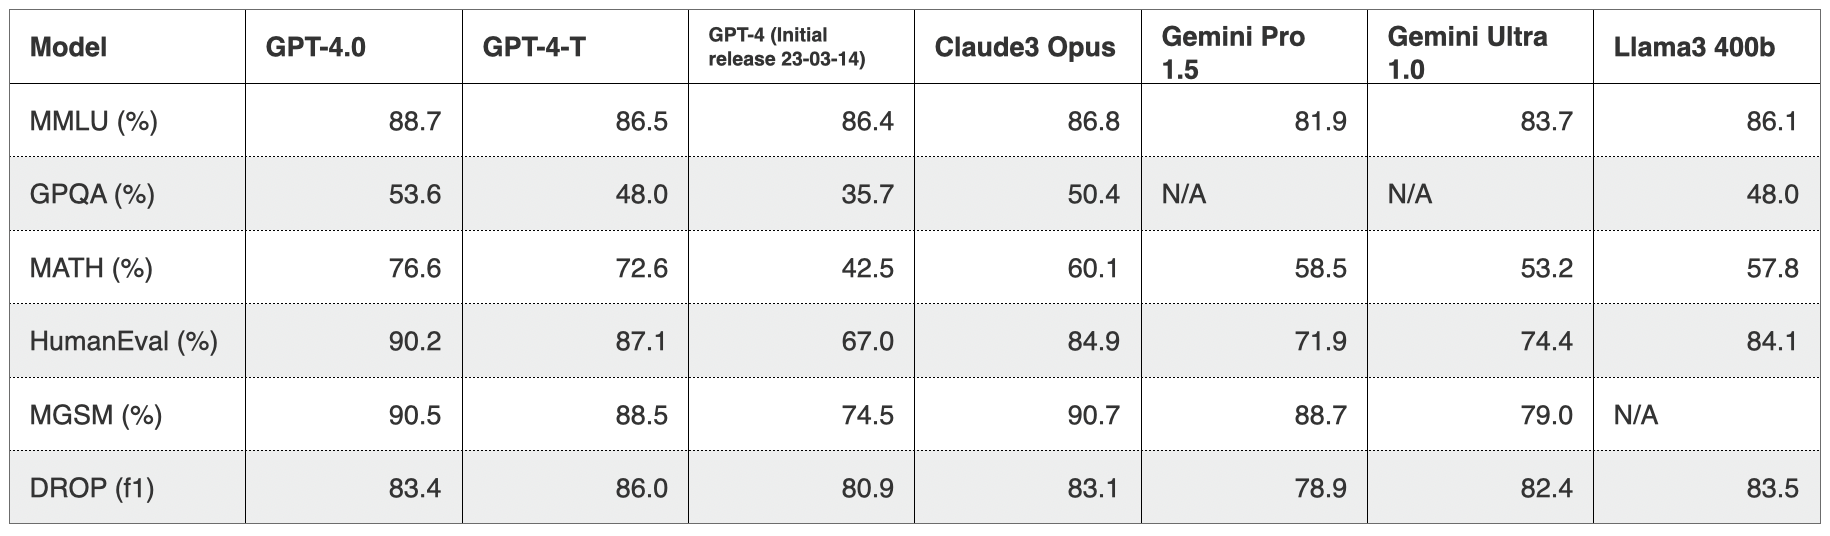
\includegraphics[width=0.75\linewidth]{figures/case/case1-2.png}
  \end{center} \\
  
  \midrule
  
  \begin{center}
  
\includegraphics[width=0.55\linewidth]{figures/case/case2.png}
  \end{center} \\
  {\footnotesize\textbf{Instruction:} Answer the question in image.} \\
  {\footnotesize \textbf{\mimovlrl{}:} \texttt{<think>...</think>} To solve for the tension in the wire, we use the \textbf{equilibrium of torques} about the hinge point $ P $. For a beam in equilibrium, the sum of clockwise torques equals the sum of counterclockwise torques.  

\textbf{Step 1: Identify Forces and Torques}

\quad - Beam’s weight ($ 425 \, \text{N} $): Acts downward at the beam’s midpoint (since it is uniform). The beam’s length is $ 8.4 \, \text{m} $, so the midpoint is $ \frac{8.4}{2} = 4.2 \, \text{m} $ from $ P $.  

\quad - Block’s weight ($ 720 \, \text{N} $): Acts downward at $ 8.4 \, \text{m} $ from $ P $. 

\quad - Tension in the wire ($ T $): Acts at $ 3.4 \, \text{m} $ from $ P $ at an angle of $ 23^\circ $ above the horizontal. Only the \textbf{vertical component} of tension ($ T \sin 23^\circ $) contributes to torque (the horizontal component acts along the beam, so its torque about $ P $ is zero).  


\textbf{Step 2: Calculate Torques}

Torque is defined as $ \text{force} \times \text{perpendicular distance from pivot} $.  

\quad - Clockwise torques (from the beam and block weights):  
  - Beam’s weight: $ 425 \, \text{N} \times 4.2 \, \text{m} = 1785 \, \text{N·m} $  
  - Block’s weight: $ 720 \, \text{N} \times 8.4 \, \text{m} = 6048 \, \text{N·m} $  
  - Total clockwise torque: $ 1785 + 6048 = 7833 \, \text{N·m} $  

\quad - Counterclockwise torque (from tension’s vertical component):  
  - Tension’s vertical component: $ T \sin 23^\circ $  
  - Perpendicular distance from $ P $ to the wire: $ 3.4 \, \text{m} $  
  - Torque from tension: $ T \sin 23^\circ \times 3.4 \, \text{m} $  


\textbf{Step 3: Solve for Tension} 

In equilibrium, clockwise torque = counterclockwise torque:  
$
T \sin 23^\circ \times 3.4 = 7833
$  

Solve for $ T $:  
$
T = \frac{7833}{3.4 \times \sin 23^\circ}
$  

Using $ \sin 23^\circ \approx 0.3907 $:  
$
T = \frac{7833}{3.4 \times 0.3907} \approx \frac{7833}{1.328} \approx 5900 \, \text{N}
$  


\textbf{Final Answer}  
The tension in the wire is approximately $ \boldsymbol{5900 \, \text{N}} $.
}\\
  \bottomrule
  \end{tabular}\\
\caption{Examples of \mimovl{} solving complicated problems.}
\label{fig:case_main}
\end{figure}


\subsection{Interference Between RL Tasks}
While MORL training enhances performance on nearly all evaluated tasks, achieving stable and simultaneous improvements across diverse task domains remains a significant challenge.
During training, we observe that reasoning tasks exhibit disparities with visual perception and grounding tasks, such as visual grounding and counting, making it difficult to match the performance of standalone RL on individual tasks.

The potential cause lies in the opposing growth trends of response length: reasoning tasks encourage longer CoT during the RL process, whereas grounding and counting tasks lead to shrinking ones.
Disparities in task difficulty and the risk of reward hacking may also contribute to this interference.
We are actively investigating the underlying causes of this phenomenon and seeking solutions to achieve consistent and persistent growth across all tasks.




\section{Case Study}

\begin{figure}[!htbp]
    \centering
    \includegraphics[width=0.95\linewidth]{figures/gui_case.pdf}
    \caption{A case demonstrating the agentic capabilities of our model. \mimovl{} successfully navigates a website to add the Xiaomi SU7 to the wishlist, customizing both paint and interior options. All screenshots are of size 1886*1544 (width*height).}
    \label{fig:gui_case}
\end{figure}

We present qualitative results in Figure~\ref{fig:case_main} and Appendix~\ref{sec:more_cases}.
As depicted in the top example in Figure~\ref{fig:case_main}, our model showcases strong plot understanding capabilities, successfully converting an intricate plot into a well-structured markdown table.
Additionally, we highlight the models' superior reasoning capabilities in STEM tasks.
In the examples shown in Figure~\ref{fig:case1} and Figure~\ref{fig:case4}, the model effectively addresses multiple STEM questions within a single response.
Furthermore, our model exhibits strong agentic capabilities.
As illustrated in Figure~\ref{fig:gui_case}, \mimovl{} successfully navigates a website to add the Xiaomi SU7 to the wishlist, with customized paint and interior options.




